\section{Benchmark Datasets}
This section will outline some of the commonly used object detection datasets. This will include their purpose and the general setup.


\subsection{PASCAL Visual Object Classes Challenge}
The \gls{pascalvoc} challenge \cite{pascalvoc2012} was held yearly between 2005 to 2012 and provided datasets for benchmarking within vision tasks of visual object category recognition and detection. Between that time period is was considered the top benchmark for the respective challenges. While being an annual competition, \gls{pascalvoc} evaluation in state-of-the-art literature is most often performed on data from the years 2007 and 2012. The competition saw a large shift in the former year as the number of classes increased from 10 to 20, in turn also significantly increasing the total amount of data. Additional data was added individually for the various recognition tasks between 2007 and 2012 and the performance metric was altered slightly between this time period, however, the overall ecosystem remained largely the same from 2007 until the competition's end. This section will be largely based upon the two retrospective papers, \cite{pascalvoc2010} and \cite{pascalvoc2015}, published by authors who were involved in the challenge and for the most part will be in respect to the challenge after 2007.
\\\\
Images were obtained from the website flickr \cite{flickr} with the aim in mind to collect natural images for the recognition challenges. Ideally the dataset was to contain a significant level of visual variability in regards to object size, orientation, pose, illumination, position, and occlusion. A total of 20 classes were present in the 2007 challenges and these remained the same until 2012. The classes can be considered as a part of a taxonomy with 4 main branches, where each has finer-grain objects in sub-classes. The 20 classes and the branching taxonomy can be seen in \tableref{vocclasses}.


\begin{table}[h]
\centering
\caption{Taxonomy of the 20 classes introduced in VOC2007.}
\label{tab:vocclasses}
\begin{tabular}{llll}
\hline
Vehicles & Household & Animals & Other \\ \hline
Aeroplane                      & Bottle                         & Bird                         & Person                     \\
Bicycle                        & Chair                          & Cat                          &                            \\
Boat                           & Dining table                   & Cow                          &                            \\
Bus                            & Potted plant                   & Dog                          &                            \\
Car                            & Sofa                           & Horse                        &                            \\
Motorbike                      & TV/Monitor                     & Sheep                        &                            \\ \hline
Train    &  &  &  \\ \hline
\end{tabular}
\end{table}

A total of 500,000 potential images were collected randomly based upon different combinations of queries for a given class. For example of class bird, potential queries were bird, birdie, birdwatching, nest, sea, aviary, birdcage, bird feeder, and bird table. Of these potential images the majority were discarded for potential annotation due to not meeting the considerations of visual variability mentioned earlier. The annotation process was completed by a team from the University of Leeds based upon strict guidelines. The aim was to ensure that the annotations resulted in a consistent, accurate, and exhaustive dataset. The annotations are stored in XML format which contains the following information:

\begin{itemize}
	\item Class: one of the 20 shown in \tableref{vocclasses}.
	\item Bounding box: axis-aligned bounding-box around the visual extent of the object.
	\item Viewpoint: viewpoint to the object.
	\item Truncation: whether or not object is truncated. An object is truncated when the bounding-box does not cover the full extent of the object. Truncation can occur if the object extends outside the image or is partially occluded.
	\item Difficult: A subjective evaluation on if the object is difficult to detect. This is determined based on object size, illumination, or image quality.
\end{itemize}

An example of the XML format for the object chair can be seen in Code \ref{lst:xml_ex} and its corresponding image in \figref{xml_eximg}. 

\begin{lstlisting}[language=xml,caption={Example of XML annotation for the object chair.}
\label{lst:xml_ex}]
<object>
    <name>chair</name>
    <pose>Rear</pose>
    <truncated>0</truncated>
	<difficult>0</difficult>
	<bndbox>
		<xmin>263</xmin>
		<ymin>211</ymin>
		<xmax>324</xmax>
		<ymax>339</ymax>
	</bndbox>
</object>
\end{lstlisting}

\begin{figure}[H]
  \centering
    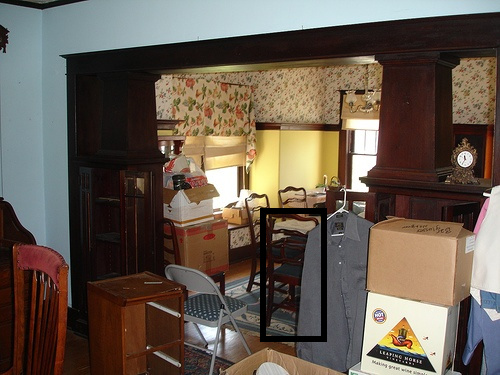
\includegraphics[width=0.7\textwidth]{Figs/Techanal/000005.jpg}
    \caption{Image from the \gls{pascalvoc} 2007 dataset. The bounding box represents the annotated XML data shown in Code \ref{lst:xml_ex}.}
    \label{fig:xml_eximg}
\end{figure}

Of the 500,000 potential images, 9,963 were annotated for the VOC2007 challenges based upon the annotation guidelines. \gls{pascalvoc} datasets is split into two subsets; \lstinline{trainval}, consisting of training and validation data and \lstinline{test}, consisting of the testing data. A histogram showing the frequency of an object class in an image and the total number of objects for the VOC2007 dataset can be seen in \figref{vochist07}.

\begin{figure}[H]
  \centering
    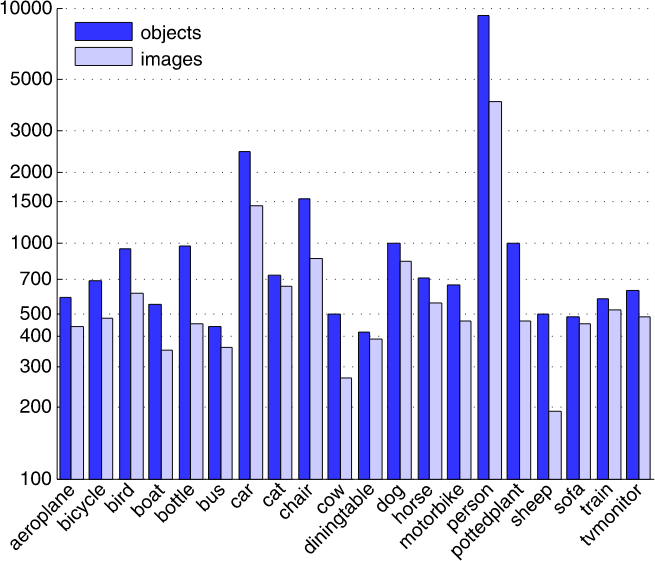
\includegraphics[width=0.5\textwidth]{Figs/Techanal/vochist07.png}
    \caption{Image from the \gls{pascalvoc} 2007 dataset. The bounding box represents the annotated XML data shown in Code \ref{lst:vochist07}.}
    \label{fig:vochist07}
\end{figure}




Evaluation of a object detector on \gls{pascalvoc} is based upon \gls{ap} which summarises the precision and recall of detections. The metric requires that for each detection both a bounding-box and an associated confidence. With these a precision/curve can be calculated and the overall \gls{ap} for the curve represents the performance of the detector. Firstly, the bounding-box